\documentclass[conference]{IEEEtran}
\IEEEoverridecommandlockouts
% The preceding line is only needed to identify funding in the first footnote.  If that is unneeded, please comment it out.
\usepackage{cite}
\usepackage{amsmath,amssymb,amsfonts}
\usepackage{algorithmic}
\usepackage{textcomp}
\usepackage{xcolor}
\def\BibTeX{{\rm B\kern-.05em{\sc i\kern-.025em b}\kern-.08em
    T\kern-.1667em\lower.7ex\hbox{E}\kern-.125emX}}

\usepackage{a4wide}
\usepackage{makeidx}
\usepackage{times}
\usepackage{epsf}
\usepackage{graphicx}
\usepackage{epsfig}
\usepackage{graphics}
\usepackage{color}
\usepackage{url}

\usepackage[english]{babel} % otherwise, \cite doesn't work with sig-alternate/acm_proc_article-sp
\usepackage{txfonts}
%\usepackage{multiFloats}

\usepackage{pslatex}
\usepackage[all]{xy}

%% wrap text around (floating) figures
\usepackage{wrapfig}
%%\setlength{\wrapoverhang}{0mm}

\begin{document}

\title{Database Resource Allocation Based on Resident Intermediates}

\author{
\IEEEauthorblockN{Martin Kersten, Panagiotis Koutsourakis, Joeri van Ruth, Ying Zhang}
\IEEEauthorblockA{
\textit{MonetDB Solutions}\\
Amsterdam, The Netherlands \\
<lastname>@monetdbsolutions.com}
}

\maketitle

\begin{abstract} 
%What is the market pitch? 
Scale-out of big data analytics applications often does not pay off due to the poor response time performance and the bill ticking for a longer time on a resource limited machine.
In a stable DBMS workload environment it helps to maintain several virtual machines hosting
part of the database and sending the tasks to those machines that have the best price/performance characteristics.
This, however, requires a method to learn over time which VM should be charged with the
query and the technology needed is the focus of this paper.
\end{abstract} 

\section{Introduction}
\label{Introduction} 
Since its inception, database designers have keenly looked at the opportunities to use large, distributed processing platforms. Cluster-based products are readily available, but are often limited to a few tens of compute nodes and call for a strong engineering to avoid hardware bottlenecks, such as in appliance products from Oracle Exadata, SQL Parallel Data Warehouse, and IBM Blu and Teradata.

A plethora of research activities have shows that in all but the simplest cases, achieving a good performance is at least very hard. Especially when the query involves joins spread over multiple compute nodes and require an expensive data exchange. 

The predominant way out, taken in NoSQL systems  \cite{Casandra,Impala} is to address part of the problem space by focusing on select-aggregate queries. This focus on part of the problem space for distributed query processing has been shown pivotal to support big-data analytics in many real-world circumstances, as shown by the widespread use of Apache Spark \cite{}, which is widely used nowadays to encode distributed applications.
The basic abstraction in Spark is a Resilient Distributed Dataset (RDD), which represents an immutable, partitioned collection of elements that can be operated on in parallel using operators, such as map, filter, persist and aggregates. Moreover, the RDD is the basic component to exchange between operators, threads, cores and machines. In essence, an RDD can be seen as a relational table used for interoperability, an approach that can be traced back to Microsoft's ODE \cite{} used for decades to exchange data between DBMS and applications. Similar functional abstractions can nowadays be found in R's Dataframes and Python Pandas\cite{}.

%explain the former tells it can be re-constructed upon need.

Although in most cases, it is easy to scale-up for improved response time, partitioning a database to benefit from a low Cloud service price tag, better use of parallel IO, or resource limitations of smaller machines is still worth considering. This product space is addressed by Snowflake and AWS Redshift. Snowflakes has been designed from a Cloud perspective, taking
resource management as its key driving factor. It conceptually provides every user with a complete copy of the database and relying on multi-level caching. AWS Redshift is an improved
version of Postgresql further tuned towards better IO bandwidth.

In this paper we take a fresh look at resource allocation to query processing in the context of where intermediates in a query plan are fully materialized before passed on towards the next operator. This model fits the Apache Spark programming model, but also the query execution model underlying MonetDB. Resilient intermediates provides new avenue for query optimization and scheduling as it underlying computation model is based on materialization of all intermediate steps. Furthermore, in most practical business analytic cases the past is a reasonable predictor of the future.

The main contributions of this paper are
\begin{itemize}
	\item we develop a simulator to predict the memory footprint  for queries based on resident intermediates.
	\item We demonstrate the approach is robust against varying data distributions.
	\item We demonstrate the opportunities using an extensive evaluation against TPC-H and a real-world databases.
\end{itemize}

The approach taken differs from traditional cost-based optimizers deployed in distributed database systems by learning the resource claims over time. For, after each query step we have precise knowledge of the resources claimed. This information can be harvested and to predict future operations of a similar nature. The rational stems from the common knowledge that any database application environment has a limited number of 'business transactions' or 'BI templates' where only some parameters are changed with each call. This knowledge has been used in the past to drive development of DBA wizards \cite{microsoft} for index selection by humans and self-tuning optimizers \cite{IBM} to avoid expensive join paths in individual queries.

Outline of paper. Section \ref{Background} provides a short introduction to the MonetDB architecture and the projects involved. Section \ref{Malcolm} introduces the components
and algorithms for our resource estimator.
Section \ref{Evaluation} illustrates the effectiveness of the approach in two use-cases: TPC-H and Airtraffic.

\section{Background}
\label{Background} 
In this section we summarize the salient features of resilient intermediates for query processing.
, the leading open-source  column store and the envisioned system ExaNest, an exascale HPC platform for data-intensive computing.

\subsection{A Column Store}
%Recap some MonetDB stuff on how queries are compiled.
MonetDB is a widely used column store that internally is uses resident intermediates to break up query processing in well identifying steps. 
The query plan is broken up into independent steps, glued together into a dataflow dependency graph.  The dataflow graph is greedily consumed by the database kernel assigning a single core to a single operation. The resource pressure is kept at a minimal to trim down the degree  of parallel processing when the main resource, RAM, is heavily used.
The system can be instructed to produce an event record for each completed instruction. This provides a.o. insight into the input/output sizes and timing. 

\subsection{Distributed Query Optimizers}
% summarize 
The predominant scheme to scale out database processing is to break the base tables into independent partitions using either a hash-key or ranges. The partitioning scheme can be used to orchestrate distributed processing in an optimal way most of the time.

\section{Query Execution Model}
In this section we describe how the MonetDB query execution engine was used to develop a novel. We also illustrate the data at our disposal to predict

\subsection{Architecture}
Figure \ref{fig} illustrates the components our reference system, MonetDB, to execute an sql query. The SQL parser and optimizer layer deploy well-known rewriting rules to reduce the intermediate sizes and processing time. It does not rely on any cost-model or pre-computed statistics (aside from the whereabouts of the data partitions on separate nodes)

The middle layer is a sequence of specialized optimizers that morph the logical plan received from the SQL compiler into a physical execution plan. Constant expressions are evaluated, common sub-expressions are identified, the dataflow graph for parallel processing is derived, etc...

The bottom layer contains the implementation of the relational operators. Each operator takes as input the resident intermediates produces before or they access the persistent data on disk. The actual implementation is often quite complex, because each operator can be implemented in a multitude of ways. Since the operator has full knowledge on the actual parameters, it becomes easy to select the proper path. Some operators even perform a sampling step before making a choice on the preferred algorithm.

To illustrate consider the following simple SQL query
The actual code executed by the MonetDB kernel is shown in Figure \ref{label}. 
%clarify what you see

The details of the actual execution can be gathered using the Stethoscope. A single record is shown in Figure \ref{}. Of interest to this paper are the properties shown for the arguments and return variables.

\subsection{Profiling Information}
The MonetDB kernel can be instructed to emit profiling events. Every primitive function comes with an event record taken at the start and upon completion of the operation. The event record contains details on the arguments passed, their type and size. Where ever possible the arguments are linked with the underlying persistent column. Intermediate columns are nameless and we only can rely on their type/cardinality.
Upon completion, we also know the exact size of the result and the time consumption.
The data flow between the instruction is also available, but for the remainder of this paper ignored. We assume a worst case execution scenario where the maximum footprint is determined.

Explain a MAL instruction
For the remainder of this paper it is necessary to have a basic knowledge of the MAL programming language in which all SQL queries are translated. The MAL language is purely designed as intermediate language to express the operations 

The general format is
\begin{verbatim}
content...
\end{verbatim}
Every function belongs to a module. The arguments are either typed scalar values (:type) or a reference to a column (:bat[:type]).

In principle we should collect all possible events as a basis for building an optimizer/simulator. Although the MonetDB kernel knows $>$10K operator/type specific signatures, the SQL front-end only needs a few tens of operator templates.
For the TPC-H benchmark  ca 60 MAL operations are sufficient. Figure \ref{instructions} shows the top 20 with their relative time consumption for a run against SF10.

{\tiny\begin{verbatim} 
21.83 %       1332 calls algebra.projection
12.91 %        768 calls mat.packIncrement
 9.60 %        712 calls algebra.projectionpath
 7.58 %        558 calls sql.bind
 7.45 %        519 calls batcalc.*
 7.25 %        435 calls algebra.join
 5.48 %        330 calls bat.append
 4.52 %        420 calls algebra.thetaselect
 3.44 %        234 calls sql.bind_idxbat
 3.34 %        223 calls algebra.select
 2.49 %        179 calls sql.tid
 2.46 %        144 calls batcalc.!=
 2.06 %        138 calls aggr.subsum
 1.98 %        218 calls bat.mergecand
 1.30 %         74 calls sql.projectdelta
 1.06 %         74 calls group.groupdone
 1.06 %         75 calls bat.new
 0.92 %         53 calls batcalc.==
 0.90 %         72 calls batcalc.-
 0.78 %         39 calls batcalc.dbl
\caption{The top-20 MAL operators for TPCH\label{instructions}}
\end{verbatim}
}
\section{Micro Models}
With an abundance of events we can start to derive models for each of the instructions. A micro model is derived that can be used later for ease of simulation alternative execution plans. We study them based on similar properties.

\subsection{Load instructions}
Bind instruction loads (or memory maps) a column into memory,
thus the result size is the size of the column. This is a worst case assumption,
because in practice not all of the column needs to be loaded. For example,
if the column is sorted and we perform a range select then the size of the result
determines the footprint.

However, using the full column size aids in cache management, because over a series
of queries like it will be completely loaded.

\subsection{Arithmetic Operations}
The operations can be grouped by complexity to predict the outcome of a hypothetical operation. The first group includes the {\em batcalc} operations. They all obey the following structure:
\begin{verbatim}
  res:bat[:lng]:= batcalc.==( l:bat[:lng],r:bat[:lng])
  res:bat[:lng]:= batcalc.==( l:bat[:lng],r::lng)
  res:bat[:lng]:= batcalc.==( l:lng,r:bat[:lng])
  res:bat[:lng]:= batcalc.==( l:lng,r:lng)

\end{verbatim}
The argument is either scalar or a reference to a column. However, in all cases the number of result tuples can be looked up from the argument events. The processing time depends mostly on the type's footprint and the influence of concurrent activity.

\subsection{Filter Operations}
The next group is formed by the filter operations {\emph thetaselect, select}. In this case we know that the output is always smaller then the candidate tuples considered. But how to determine the estimated result size. Traditional cost-based models assume a uniform distribution of the data and calculate the fraction of the domain, i.e. the selectivity factor.

In our case, we have can collect a series of actual filter operation and keep them around to find a 'nearest-neighbor'. A synopsis of the search algorithm is shown in Figure \ref{.}
It initially considers two events neighbors if they relate to the same underlying persistent column. For this case the candidate lists determine how many elements are still to be consider by the filter operations.

To predict the size of a range select, we used the kNN algorithm,
using k=5, to find the 5 closest selects to the one we want to predict,
considering the lower and higher bounds as distance metrics.
When we are facing a one bound select ($<$,$>$ etc) we use the
dataset statistics to fill the other bound (e.g in case of $<$ we want the column min).

\subsubsection{Subsequent Selects}
%TODO make it more general
In case of intermediate select instructions, the ranges are not adequate to
make an accurate prediction, because the argument size may vary based on the
previous selects. To overcomes this we incorporated the estimations of the
previous intructions, to build a graph that relates each variable to a size
estimation. This way we cal also use the argument estimation to predict the
size of the select result. The code for selection prediction is shown at
Figure\ref{sel:code}. In real life it is very common to find correlated columns,
in which the first selection may affect non-linearly the second.
In our design we do not handle such cases(Future work).

\begin{figure}[t]
	\begin{verbatim}
	def div(i1, i2):
	return (i1.hi-i1.lo) / (i2.hi-i2.lo)
	
	def extrapolate(traini, testi):
	traini.cnt*div(testi,traini)*testi.approx_arg_cnt/traini.argcnt
	
	def predict(testi, traind, approxG):
	knn5 = traind.knn(testi,5)
	return sum([i.extrapolate(testi) for i in knn5]) / len(knn5)
	\end{verbatim}
	\caption{Code snippet for making predictions for range selects}
	\label{sel:code}
\end{figure}

\subsubsection{Point Selects}
Again we use the kNN to find the 5 closest points,
and extrapolate based on the argument size.
\subsubsection{Limit Operations}
Limit and sample operators(firstn, and sample? in MAL) are also trivial,
we just output the minimum of the argumens size and the limit size.

\subsection{Projection Operations}
Projection operators extract a small part of a column. The arguments are a candidate list and a reference to the (persistent) column. The number of elements is equal to the size of the candidate list and the time is based on the random access and copying the data around.

In some weird cases, the projection instruction
returns str(copies from heap) instead of ids,
which makes hard to predict. In this case, we run a kNN
based on the type and argument distance, to find a similar
instruction use this to find the output size.

\subsection{Join Operations}
In Malcolm we use a kNN(k=5) on the joins we have in our dictionary,
that operate on the same two columns if possible,
and find the ones closest based on the argument sizes.

\begin{verbatim}
content...
\end{verbatim}
Such join sequences are mostly pointer chasing activities where the result set typically is less then the smallest argument. (to be checked)

\subsection{Grouping Operations}
multiple operations to be considered.

\subsection{Aggregate Operations}
This category includes operations like sum, avg, min, max, single, dec\_round
The count of the result is obviously one.

The groupby signature is:
\begin{verbatim}
(bat[:oid], bat[:oid], bat[:X]) := group.groupdone(bat[:X]);
\end{verbatim}
The first return value is the ids of the grouped column, the second is
the ids of the discinct values of the column(the third what ??). To predict
the size of the return variables, we use the ground statistics of the column
(size, count, discinct values).

The operation subgroupdone has a similar signature to groupdone, but it operates on intermediate
variables, where we do not have the column information. In this case, we run a
kNN based on the argument sizes.

Orderby is translated into sort in MAL.

\subsection{Set instructions}
We do not have any relevant information to do an accurate guess for the
set instructions, so we output the worst case of the result.
$$ intersect(A,B) ~= min(A,B)$$
$$ merge(A,B) ~= A+B $$
$$ diff(A,B) ~= A $$
\begin{verbatim}
(bat[:X],bat[:oid],bat[:oid]) := algebra.sort(bat[:X], bat[:oid], bat[:oid], bit, bit)
\end{verbatim}
The size of each return value is exactly the same as the corresponding argument size.

\subsection{Limit Operations}
Limit and sample operators(firstn, and sample? in MAL) are also trivial,
we just output the minimum of the argumens size and the limit size.

\section{Optimizer Simulator Architecture}
With the micro-models in place, we can use a simple MAL-simulator to obtain a precise indication of the memory footprint. In its basic form it simulates a sequential execution of the query. The full-blown version uses the same scheduling method as within the MonetDB code base to approximate the parallel behavior.

\section{Evaluation}
In this section we show how the footprint predictor works based on an increasing event list.
To conduct our experiments we used both TPC-H and the Airtraffic benchmarks. The former is
the baseline against which most database systems are evaluated. Its major weakness is the
uniform data distribution. Although this simplifies analysis of the quality of a space
predictor, it is not representative for a real-life case. Therefore, we also use the airtraffic
benchmark~\cite{airtraffic}, which consists of a single table with $>$ 120 M rows and 100 columns of flight information. The data is skewed.


\subsection{TPC-H}
To exercise Malcolm against TPC-H we created a query generator, which changes the parameters in the official benchmark. A key factor in the design of Malcolm is to understand how long it
takes before it has 'learned' the data distribution and how precise it will be. Therefore, we
used a large collection of morphed queries and split it two portion. One part is used to
feed into the simulator to learn the data distrution, while the second part is used to assess
the quality.

Initial experiments led to the results shown in Figure~\ref{fig:overviewQ1} and ~\ref{fig:overviewQ2}. TPC-H is a simple large scan followed by an aggregation. 
The parameter is the value range. The experiment shows a steep learning curve, which can be
attributed to the uniform distribution. However, it also results in a little over fitting.

As a training set for each query, we randomized every selection point and range,
and produced 200 random versions of the query. As a test set we used the original
query.

In query 19 we observe a misprediction of 70\%. The reason this happens, is that
the MAL algebra of this specific query consists of a lot of merge instructions,
for which we output the sum of the two arguments, which in case of merging similar
variables can lead to an almost 2$\times$ overestimation.
This is the basic reason for the large error observed.
\begin{verbatim}
culprit:
C_187 := algebra.thetaselect(X_178, "DELIVER IN PERSON", "==");                                                                                                                                                                                                                    |
X_191 := bat.mergecand(C_187, C_187);                                                                                                                                                                                                                                              |
X_194 := bat.mergecand(X_191, C_187);
\end{verbatim}
[Move queries to appendix]
\begin{verbatim}
select
l_returnflag,
l_linestatus,
sum(l_quantity) as sum_qty,
sum(l_extendedprice) as sum_base_price,
sum(l_extendedprice * (1 - l_discount)) as sum_disc_price,
sum(l_extendedprice * (1 - l_discount) * (1 + l_tax)) as sum_charge,
avg(l_quantity) as avg_qty,
avg(l_extendedprice) as avg_price,
avg(l_discount) as avg_disc,
count(*) as count_order
from
lineitem
where
l_shipdate <= date '1998-12-01' - interval '90' day (3)
group by
l_returnflag,
l_linestatus
order by
l_returnflag,
l_linestatus;
\end{verbatim}

TPC-H query 6 is also mostly a simple scan and aggregate query, but here the number of
tuples are less. This experiment that Malcolm takes much longer to reach an almost perfect
prediction of the memory footprint.

\begin{verbatim}
select
sum(l_extendedprice * l_discount) as revenue
from
lineitem
where
l_shipdate >= date '1994-01-01'
and l_shipdate < date '1994-01-01' + interval '1' year
and l_discount between .06 - 0.01 and .06 + 0.01
and l_quantity < 24;
\end{verbatim}

\begin{figure}[t!]
	\centering
	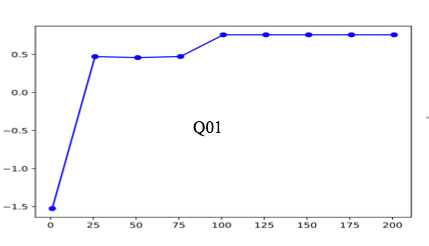
\includegraphics[height=2in,width=3in]{Figures/Q1.png}
	\caption{TPC-H Query 1 error bounds
		\label{fig:q1}}
\end{figure}

\begin{figure}[t!]
	\centering
	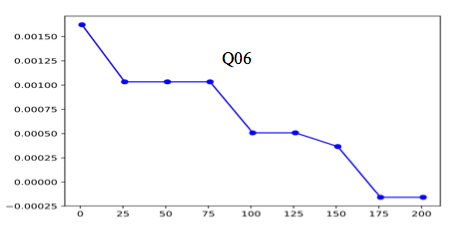
\includegraphics[height=2in,width=3in]{Figures/Q6.png}
	\caption{TPC-H Query 6 error bounds
		\label{fig:q6}}
\end{figure}


\subsection{Airtraffic}
The Airtraffic benchmark is a real-world example of  business intelligence application.
Although it is represented by a single table, it is highly skewed and sparse. The queries
are mostly simple select-group-aggregate, but given the table size still hard to process.
Again we can see both an under-estimate and an over-estimate that improve over time.
One immediate observation is that in this case it takes more queries to reach an optimal
estimate. One with a low error rate.
Figure ~\ref{fig:4-15}for query 4  also illustrates how Malcolm not necessarily monotonically
improve. Of course, this is a result of the query load.
\begin{figure}[t!]
	\centering
	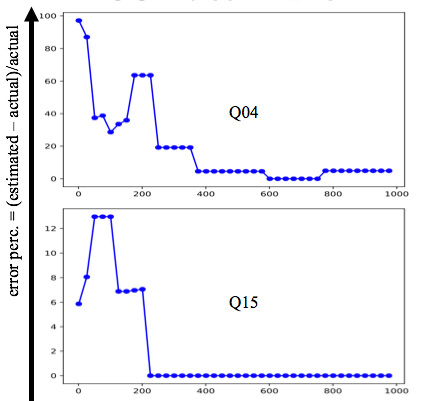
\includegraphics[height=2in,width=3in]{Figures/Q4-15.png}
	\caption{Airtraffic query 4 and 15
		\label{fig:4-15}}
\end{figure}

\begin{figure}[t!]
	\centering
	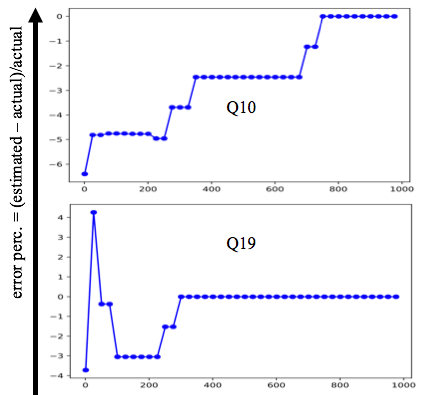
\includegraphics[height=2in,width=3in]{Figures/Q10-19.png}
	\caption{Airtraffic query10 and 19
		\label{fig:q10-19}}
\end{figure}

\section{Related work}
The approach taken in this project can best be compared with the long tradition in database
query optimizers and database design wizards. They all collect query traces from an actual production system and use them
to derive e.g. an optimal set of search accelerators \cite{DBLP:conf/vldb/ChaudhuriN07}. This process seeks a balance between index creation and maintenance, but primarily deals with
performance optimization. The memory footprint is of less concern.
Alternatively, it extends the work on gathering query traces to (semi) automatically improve the cost model for query
optimization \cite{DBLP:journals/ibmsj/MarklLR03}. A better statistics improves
both performance and resource use.
All these systems are focused on a relative small and fixed compute cluster or database 
appliance.

In a more recent project \cite{DBLP:journals/pvldb/DingDWCN18} the authors gather sub-plans from the 
query trace log and use it as the building block for new queries. They show that
re-use of good plans, i.e. based on past behavior, leads to both a faster optimization
step and overall better performance. Malcom does not address the optimizer itself, but
assumes that a physical plan has already been produced. It merely determines which
virtual machine can handle it comfortably.

\section{Summary and outlook\label{summary}} 
In this paper we proposed a novel resource allocation 
technique for fully-materialized subqueries database
engines
 described work in progress on Malcolm,
a crucial tool in the design of Cloud-based database management solution.
The initial results are promising, a rather low number of queries are
sufficient to get a good memory footprint estimate.

In the near future, we plan to extend Malcolm to also look at the
memory footprint in relationship of the parallel execution. This should
lead to a lower bound on the memory footprint at the cost of running slower.
Both memory footprint and degree of parallelism enables the user to optimize
his system based on dollar/responsetimes.

\subsection*{Acknowledgments} This research has received funding from the European Union’s Horizon 2020 research and innovation programme under Grant Agreement no. 732366 (ACTiCLOUD).
\bibliographystyle{IEEEtran}
\bibliography{refs}

\end{document}
